
% File acl2020.tex
%
%% Based on the style files for ACL 2020, which were
%% Based on the style files for ACL 2018, NAACL 2018/19, which were
%% Based on the style files for ACL-2015, with some improvements
%  taken from the NAACL-2016 style
%% Based on the style files for ACL-2014, which were, in turn,
%% based on ACL-2013, ACL-2012, ACL-2011, ACL-2010, ACL-IJCNLP-2009,
%% EACL-2009, IJCNLP-2008...
%% Based on the style files for EACL 2006 by 
%%e.agirre@ehu.es or Sergi.Balari@uab.es
%% and that of ACL 08 by Joakim Nivre and Noah Smith

\documentclass[11pt,a4paper]{article}
\usepackage[hyperref]{acl2020}
\usepackage{times}
\usepackage{graphicx}
\usepackage{subfig}
\usepackage{latexsym}
\usepackage{float}
\usepackage{placeins}
\usepackage{booktabs}
\renewcommand{\UrlFont}{\ttfamily\small}

% This is not strictly necessary, and may be commented out,
% but it will improve the layout of the manuscript,
% and will typically save some space.
\usepackage{microtype}

\aclfinalcopy % Uncomment this line for the final submission
%\def\aclpaperid{***} %  Enter the acl Paper ID here

%\setlength\titlebox{5cm}
% You can expand the titlebox if you need extra space
% to show all the authors. Please do not make the titlebox
% smaller than 5cm (the original size); we will check this
% in the camera-ready version and ask you to change it back.

\newcommand\BibTeX{B\textsc{ib}\TeX}

%%%%%%%%%%%%%%%%%%%%%%%%%%%%%%%%%%%%%%%%%%%%%%%%%%%%

\title{CS272 Hw3: Part of Speech and Entity Recognition Sequence Tagging
with Viterbi Parsing and Per-label Evaluation}

\author{Sam Showalter \\
  University of California, Irvine \ (showalte) \\  
  Kaggle: Sam Showalter \\
\texttt{showalte@uci.edu}} 

\date{}

%%%%%%%%%%%%%%%%%%%%%%%%%%%%%%%%%%%%%%%%%%%%%%%%%%%%

\begin{document}
\maketitle
\begin{abstract}
  Part of speech tagging (POS) and entity recognition (ER) are essential tasks in natural 
  language processing. Over time, language models have evolved substantially in their 
  ability to incorporate context to leverage in accomplishing these objectives. Many 
  variations of language models for this purpose exist today, and in this study we examine 
  different configurations on a POS and NER dataset from Twitter. In addition, we develop
  a per-label evaluation metric to allow for more granular exploration of our findings. Finally,
  we implement Viterbi parsing, which uses dynamic programming to determine the most likely 
  sequence of tags using dynamic programming.
\end{abstract}


%%%%%%%%%%%%%%%%%%%%%%%%%%%%%%%%%%%%%%%%%%%%%%%%%%%%
% Introduction
%%%%%%%%%%%%%%%%%%%%%%%%%%%%%%%%%%%%%%%%%%%%%%%%%%%%
\section{Introduction}

Language models for POS and NER tagging take many forms. Initially, models relied on
window-based context that only considered a set of words directly adjacent to the 
token in question. Quickly, researchers determined that this approach would be infeasible for
capturing context over a long sequence, which occurs frequently in most languages. Therefore, 
a major revolution came from the first proposal of a recurrent, or auto-regressive network (RNN) that could carry forward its hidden state and allow it to influence the outcomes of future predictions in the sequence. Unfortunately, the most basic formulation of RNNs suffers from vanishing and exploding gradients - as a signal is passed through a sequence and subsequently propogated back during learning, the gradient tends to vanish or explode if the eigenvalues of the weight matrix is not quite close to one \cite{hochreiter1998vanishing}.

To remedy this, many ideas were proposed including gradient clipping and skip-connections, which could allow a signal to bypass parts of the sequence \cite{hochreiter1998vanishing}. Though these ideas did help, the next big breakthrough in sequence tagging and language modeling came with the idea of gating recurrent cells \cite{chung2014empirical}. That is, providing a set of parameters and strucutre that would allow the model to learn to limit context from the previous cells when it is not useful. One formulation of this, the Gated Recurrent Unit (GRU), became popular for this task. Shortly after, a more complicated but powerful variation of gating and context came from a unit known as the Long-Short Term Memory (LSTM) unit \cite{huang2015bidirectional}. Until recently, LSTM networks and their variations were considered to be state of the art. One of their notable pitfalls is there inability to be highly parallelized due to their sequential nature. This was changed by the notion of self-attention \cite{vaswani2017attention}, which dynamically computes attention and context in a parallelized fashion, leading to the enormously powerful language models known as Transformers that we see today.

Building on these ideas further, the next insight gained realized that a knowledge of the sequence predictions was necessary to ensure that the overall sequence prediction was coherent. Independently predicting labels in a sequence often leads to poor overall coherence for many tasks. Therefore, the notion of Viterbi parsing, which dynamically evaluates the most probable sequence, began to proliferate \cite{ma2016end}. In our following sections, we will walk through our custom evaluation metrics, our Viterbi parser, and our findings on POS and NER experiments with different configurations.


%%%%%%%%%%%%%%%%%%%%%%%%%%%%%%%%%%%%%%%%%%%%%%%%%%%%
% Custom Evaluation Metric
%%%%%%%%%%%%%%%%%%%%%%%%%%%%%%%%%%%%%%%%%%%%%%%%%%%%

\section{Per Label Evaluation}%
\label{sec:per_label_evaluation}

Aggregate metrics often to not capture the granularity in performance needed to evaluate a 
model in a real-world setting. Therefore, we created code that stratifies our predictions
based on their true label and computes performance metrics - in this case, accuracy - for every label. To see our code implementation, please refer to \texttt{metric.py}. This implementation passes the metric test.

%%%%%%%%%%%%%%%%%%%%%%%%%%%%%%%%%%%%%%%%%%%%%%%%%%%%
% Viterbi Parsing
%%%%%%%%%%%%%%%%%%%%%%%%%%%%%%%%%%%%%%%%%%%%%%%%%%%%
\section{Viterbi Parsing}%
\label{sec:viterbi_parsing}

One way to interpret a sequence and the operations conducted on it by a language model is as a graph where nodes are the tokens and their structural relationship (as defined by the model) are the edges. This is also know as a conditional random field, which we can use to ensure that our final sequence is coherent and incorporates the joint likelihood of the full sequence instead of independent likelihoods per term. 

For each token, we receive a transition and emission score. The emission score is the likelihood of the predicted label for that token based on the input and, depending on the model, the hidden state (context) previous to it. Conversely, the transition score is the likelihood of seeing a given emission (prediction), given the emissions previous to it. This term can be thought of as the overall coherence in the labels. With these terms together, we can find the most probable sequence using Viterbi parsing, a form of dynamic programming.

To start, initialize a matrix of scores to some default value, perhaps negative infinity. This matrix considers all labels (L) across the length of the sequence (N). Then, we also consider a (NxL) matrix of emission scores, with L scores (one per label) for each token in the sequence N. Transition scores from all labels to the others, an LxL matrix, as well as the vector of transition starting and ending scores (starting or ending with a specific label) are also probided. Lastly, we need to create another (NxL) matrix that will dynamically track the most likely sequence elements. We call this \texttt{bp} or backward pointer.

To begin, the first row of the R matrix (NxL) is seeded with the sum of the starting (predicted) label transition scores plus the emission scores for the first label. Then we iterate through the sequence of N terms, building up scores in the following way. Within the sequence loop, we iterate through the labels. We then iterate on the labels a second time, allowing us to consider all of the (LxL) possible ways options for the next most probable term in the sequence. We calculate this dynamically by finding the most probably first term, then building on it dynamically with R. We proceed in this fashion, updating R and bp during each LxL inner loop with the most probably next term. Once finished, we need to add the end transition scores. 

Finally, we can recover our most probably sequence. First, we find the highest score in the bottom row of R. This represents the end of our most probably sequence. Then, we can track backward through bp to recover the labels of this most probable sequence and return them in order. When run, this algorithm passes the Viterbi test with 100\% accuracy.


%%%%%%%%%%%%%%%%%%%%%%%%%%%%%%%%%%%%%%%%%%%%%%%%%%%%
% POS Tagging
%%%%%%%%%%%%%%%%%%%%%%%%%%%%%%%%%%%%%%%%%%%%%%%%%%%%
\section{Part-of-Speech Tagging Exploration}%
\label{sec:part_of_speech_tagging_exploration}

exploring different implementations of POS tagging. We were provided two models, one that made its predictions with Viterbi parsing and Conditional Random Field (CRF) assumptions, and another that naively produced a sequence without this information. We began our exploration with the latter.

First we incorporated word embeddings to improve the manner in which individual tokens were represented. We made use of GloVe for these embeddings, and saw an immediate jump in performance of over 10\%. In isolation, incorporating a more intelligent encoder, a bi-directional LSTM in this case, led to a nearly identical increate in performance for the simple tagger. Interestingly, the same experiment on the neural tagger showed a non-trivial difference in performance between adding only the embedder versus the encoder. Though the encoder is far more sophisticated than the embedding system GloVe, with far more parameters, the performance boost for POS tagging was more closely tied to dimensional embeddings than how context can be derived from them (encoding).

As a second round of experimentation, we explored how the dimensionality of the encoder impacts the performance. Adding more layers (stacking) tended to lead to worse performance and slower learning. While the slower learning could be due to the increased parameters, the worse performance is likely because the model has too much capacity for the task and overfits. Ultimately, a single layer with dimensionality 50 proved most effective for POS tagging, and this graph is shown for both a GRU- and LSTM-based encoders. Validation performance during learning was most stable with GRUs and while the GRU slightly underperformed the LSTM for the Neural POS tagger, repeated experiments with different initializations were more robust for the GRU implementation. Thus, we considered the GRU with GloVe embeddings as our best model and transitioned to per-label performance.



%%%%%%%%%%%%%%%%%%%%%%%%%%%%%%%%%%%%%%%%%%%%%%%%%%%%
% POS figures for experimentation and per-label stuff
%%%%%%%%%%%%%%%%%%%%%%%%%%%%%%%%%%%%%%%%%%%%%%%%%%%%
\FloatBarrier
\begin{figure*}[h]
  \begin{tabular}{cc}
    \subfloat{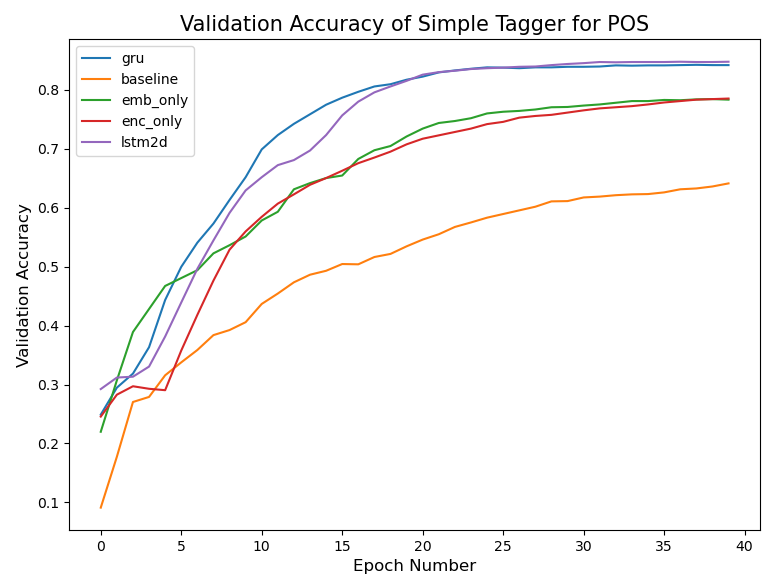
\includegraphics[width=0.48\linewidth]{imgs/val_simple_pos.png}} &
    \subfloat{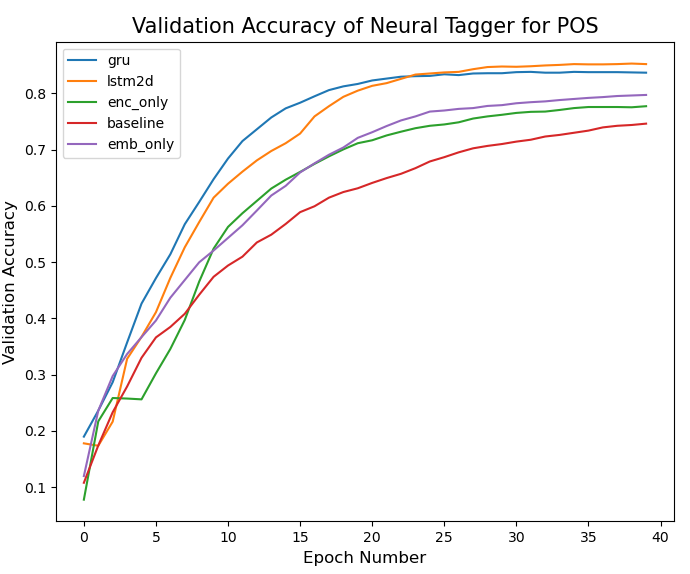
\includegraphics[width=0.44\linewidth]{imgs/val_neural_pos.png}} \\
    \subfloat{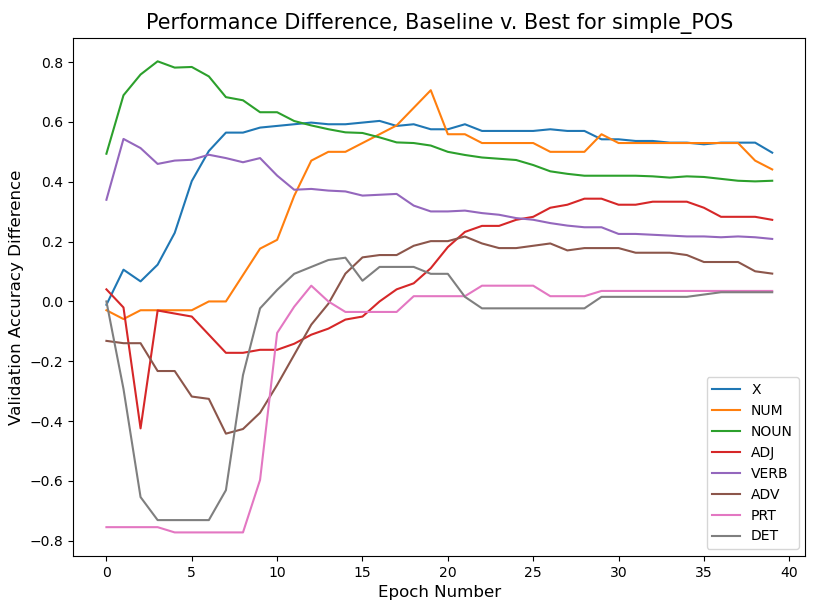
\includegraphics[width=0.45\linewidth]{imgs/label_simple_POS.png}} &
    \subfloat{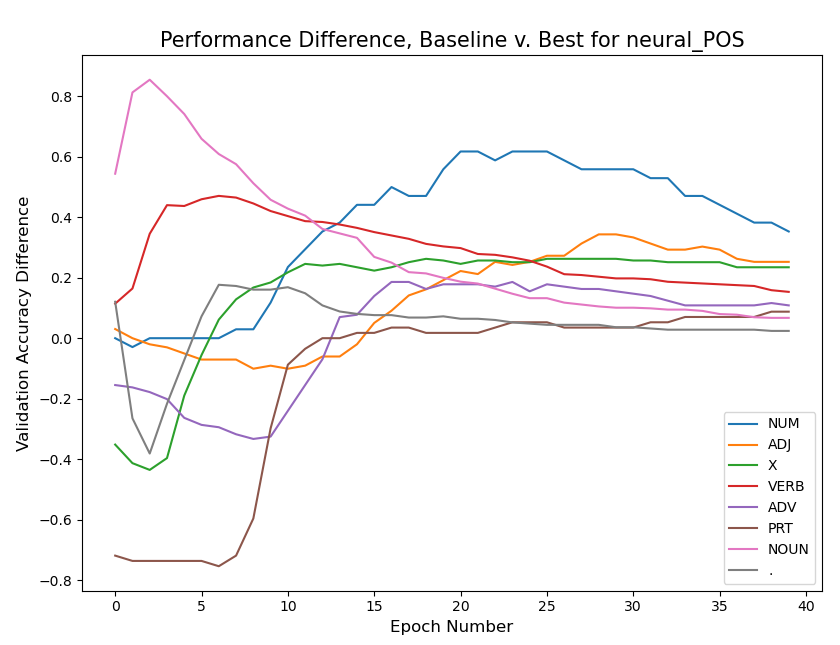
\includegraphics[width=0.45\linewidth]{imgs/label_neural_POS.png}} 
  \end{tabular}
  \caption{(Top row) POS tagging validation accuracy during training for a variety of 
    simple (left) and neural crf (right) architectures. (Bottom row) Per-label improvements 
    between baseline and best POS architectures with simple (left) and neural crf (right) 
  prediction.}
\end{figure*}
\label{fig:val_pos}
\FloatBarrier


%%%%%%%%%%%%%%%%%%%%%%%%%%%%%%%%%%%%%%%%%%%%%%%%%%%%

Displayed in the bottom row of Figure 1, the labels that benefitted the most from the GRU encoder and GloVe embeddings are similar between the neural and simple POS tagger, with \texttt{NUM} and \texttt{NOUN} tending to see the most benefit. What is more surprising is that several of these labels had performance notably worse that the baseline early on in training, only to quickly reverse later on. These similarities between neural and simple taggers continue when we consider the baseline and best models for each. Though the neural tagger baseline is substantially more performance than the simple tagger, both GRU implementations perform nearly identical to each other. It appears that the encoders we are using are particularly effective at carrying context between terms in a sequence, negating the additional performance boost from Viterbi parsing.

%%%%%%%%%%%%%%%%%%%%%%%%%%%%%%%%%%%%%%%%%%%%%%%%%%%%
% NER Tagging
%%%%%%%%%%%%%%%%%%%%%%%%%%%%%%%%%%%%%%%%%%%%%%%%%%%%
\section{Named Entity Recognition}%
\label{sec:named_entity_recognition}

%%%%%%%%%%%%%%%%%%%%%%%%%%%%%%%%%%%%%%%%%%%%%%%%%%%%
% Best POS
%%%%%%%%%%%%%%%%%%%%%%%%%%%%%%%%%%%%%%%%%%%%%%%%%%%%
\FloatBarrier
\begin{figure}[h]
  \centering
  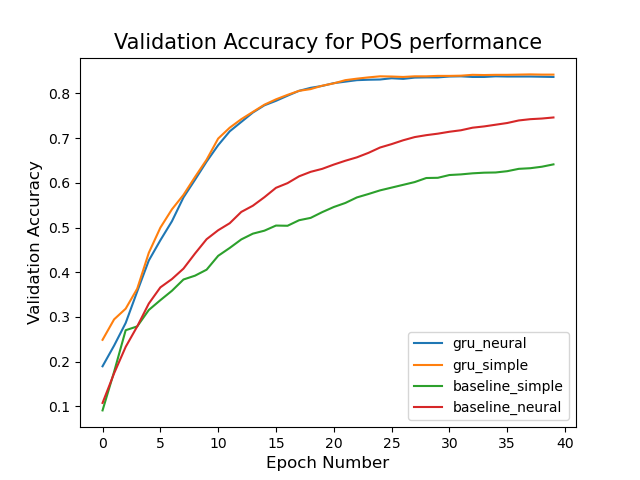
\includegraphics[width=0.97\linewidth]{imgs/best_POS.png}
  \caption{Validation accuracy for best POS models (simple and neural) as well as their
  baselines}%
  \label{fig:best_pos}
  \vspace{-13pt}
\end{figure}
\FloatBarrier
%%%%%%%%%%%%%%%%%%%%%%%%%%%%%%%%%%%%%%%%%%%%%%%%%%%%

Named Entity Resolution was a fundamentally different task than POS tagging because of the dataset imbalance. The non-named entities, labeled \texttt{'O'}, comprise a huge portion of the tokens in the dataset. In turn, one problem discovered was that the model would unanimously predict \texttt{'O'},

%%%%%%%%%%%%%%%%%%%%%%%%%%%%%%%%%%%%%%%%%%%%%%%%%%%%
% POS figures for experimentation and per-label stuff
%%%%%%%%%%%%%%%%%%%%%%%%%%%%%%%%%%%%%%%%%%%%%%%%%%%%
\FloatBarrier
\begin{figure*}[h!]
  \begin{tabular}{cc}
    \subfloat{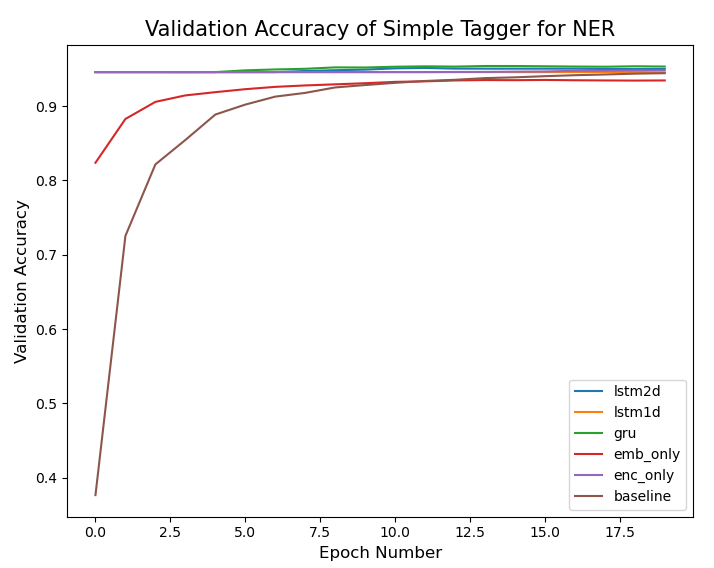
\includegraphics[width=0.48\linewidth]{imgs/val_simple_ner.png}} &
    \subfloat{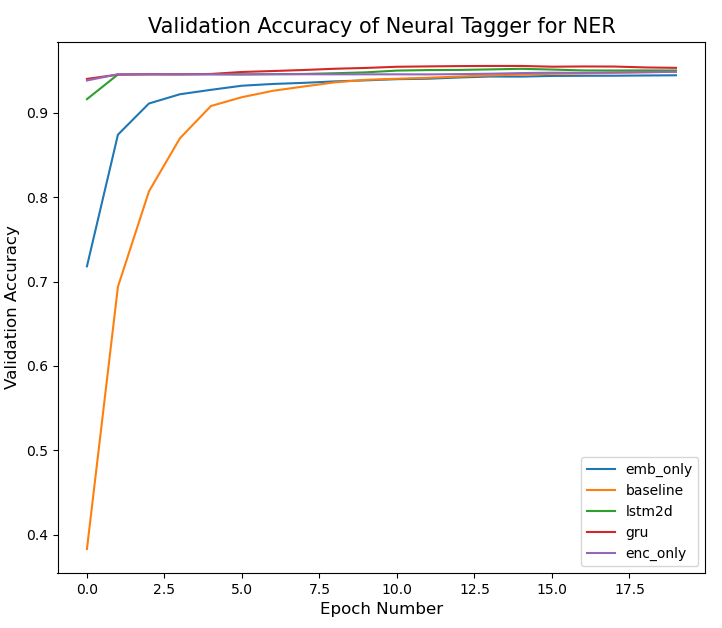
\includegraphics[width=0.44\linewidth]{imgs/val_neural_ner.png}} \\
    \subfloat{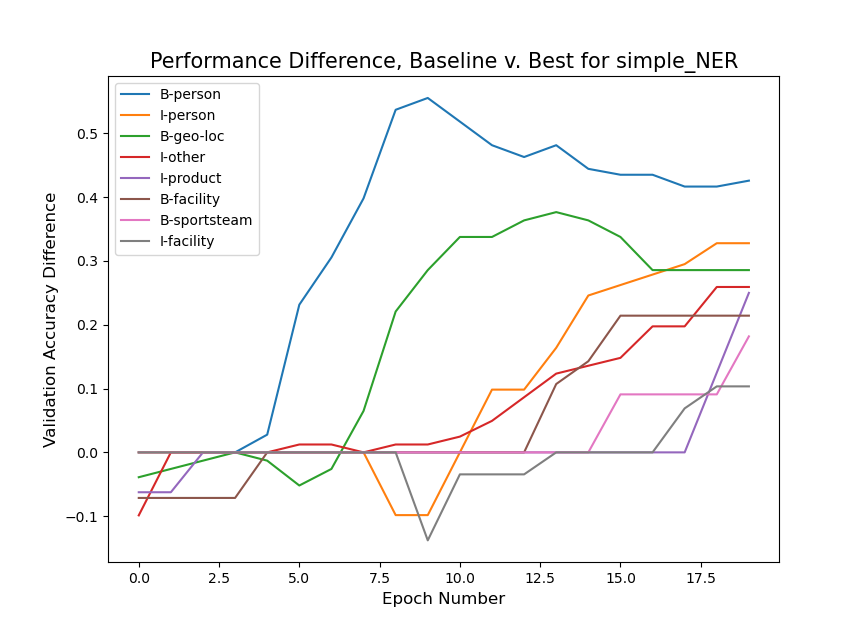
\includegraphics[width=0.51\linewidth]{imgs/label_simple_NER.png}} &
    \subfloat{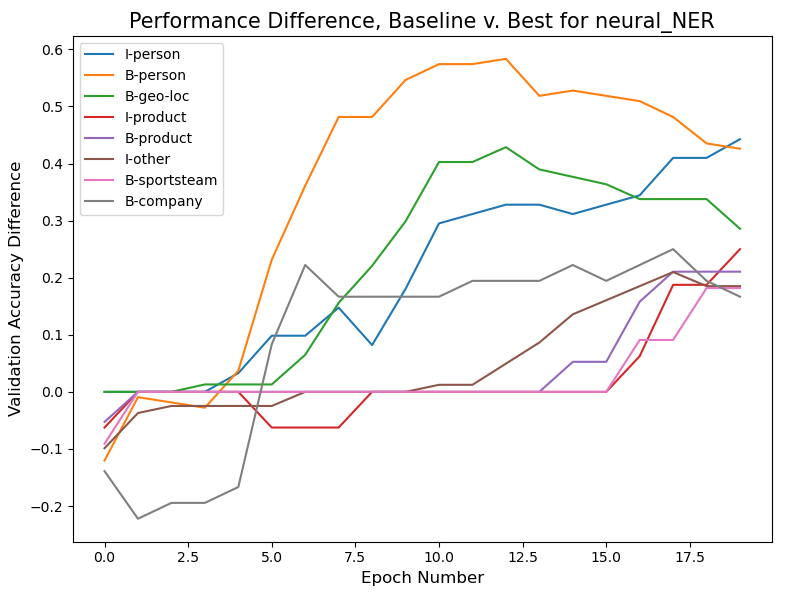
\includegraphics[width=0.46\linewidth]{imgs/label_neural_NER.png}} 
  \end{tabular}
  \caption{(Top row) NER tagging validation accuracy during training for a variety of 
    simple (left) and neural crf (right) architectures. (Bottom row) Per-label improvements 
    between baseline and best NER architectures with simple (left) and neural crf (right) 
  prediction.}
\end{figure*}
\label{fig:val_ner}
\FloatBarrier

%%%%%%%%%%%%%%%%%%%%%%%%%%%%%%%%%%%%%%%%%%%%%%%%%%%%
 leading to a decent overall performance when considered in aggregate but a poor per-label performance. Our hyperparameter tuning for NER tagging began similarly to POS tagging, which the consideration of different encoders and and embeddings separately. We also considered the impact of single-direction encoders, and have plotted the impact of a single direction LSTM in figure \ref{fig:val_ner}. Though performance was similar, one-directional encoders could not meet the performance of their bidirectional counterparts. This model was difficult to tune due to imbalanced between named and non-named entities. However, the bottom row of Figure \ref{fig:val_ner} shows the results of the final tuned models for the simple and neural CRF taggers. Again, the GRU attained the highest performance.


%%%%%%%%%%%%%%%%%%%%%%%%%%%%%%%%%%%%%%%%%%%%%%%%%%%%
% Best NER
%%%%%%%%%%%%%%%%%%%%%%%%%%%%%%%%%%%%%%%%%%%%%%%%%%%%
\begin{figure}[h!]
  \centering
  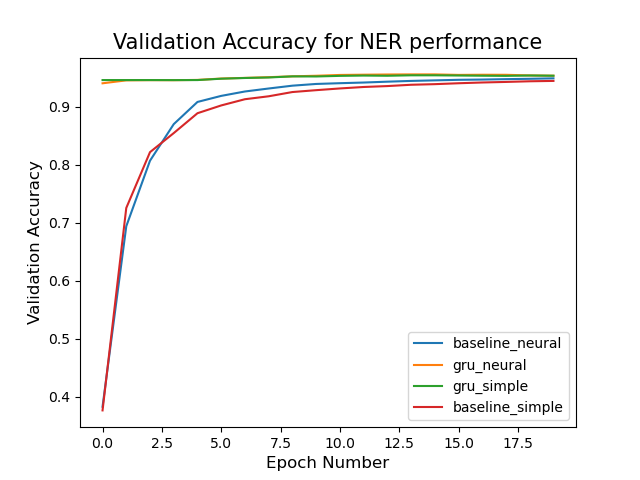
\includegraphics[width=0.97\linewidth]{imgs/best_NER.png}
  \caption{Validation accuracy for best NER models (simple and neural) as well as their
  baselines}%
  \label{fig:best_ner}
  \vspace{-16pt}
\end{figure}

%%%%%%%%%%%%%%%%%%%%%%%%%%%%%%%%%%%%%%%%%%%%%%%%%%%%

Like many of the sophisticated encoders, the GRU did struggle with predicting well over less common labels. However, it overcame this failure mode faster than other models, leading to a noticeable bump in performance per label. More interesting, however, is that the baseline performance of the NER simple and neural CRF models performed almost identically before tuning. It 

\FloatBarrier
\begin{table*}[h]
\begin{tabular}{lrrrrrrrr}
\toprule
{} &  gru\_crf &  lstm2d\_crf &  baseline\_crf &  gru\_s &  lstm2d\_s &  baseline\_s &  val\_gru\_crf &  val\_gru\_s \\
\midrule
.        &              0.96 &                 0.96 &                   0.94 &            0.96 &               0.96 &                 0.94 &             0.95 &           0.96 \\
ADJ      &              0.70 &                 0.63 &                   0.38 &            0.69 &               0.63 &                 0.41 &             0.63 &           0.64 \\
ADV      &              0.84 &                 0.82 &                   0.72 &            0.85 &               0.83 &                 0.73 &             0.69 &          0.68 \\
NOUN     &              0.76 &                 0.79 &                   0.69 &            0.76 &               0.80 &                 0.36 &             0.77 &           0.78 \\
NUM      &              0.63 &                 0.60 &                   0.25 &            0.60 &               0.61 &                 0.26 &             0.68 &           0.74 \\
PRON     &              0.96 &                 0.96 &                   0.94 &            0.96 &               0.96 &                 0.95 &             0.95 &           0.95 \\
PRT      &              0.93 &                 0.88 &                   0.85 &            0.94 &               0.88 &                 0.86 &             0.95 &           0.91 \\
VERB     &              0.87 &                 0.87 &                   0.71 &            0.87 &               0.87 &                 0.68 &             0.84 &           0.85 \\
X        &              0.82 &                 0.84 &                   0.53 &            0.82 &               0.84 &                 0.25 &             0.80 &           0.81 \\
Accuracy &              0.85 &                 0.85 &                   0.74 &            0.85 &               0.86 &                 0.63 &             0.84 &           0.84 \\
\bottomrule
\end{tabular} 
\caption{POS overall test accuracy as well as accuracy on a selection of labels. For comparison the best crf and simple validation performance are given. All scores corresopnd to the test set 
unless otherwise specified}
%\end{table*}
%\FloatBarrier

%%%%%%%%%%%%%%%%%%%%%%%%%%%%%%%%%%%%%%%%%%%%%%%%%%%%%
%% \FloatBarrier
%\begin{table*}
\vspace{12pt}
\begin{tabular}{lrrrrrrrr}
\toprule
{} &  gru\_s &  lstm2d\_s &  baseline\_s &  gru\_crf &  lstm2d\_crf &  baseline\_crf &  val\_gru\_s &  val\_gru\_crf \\
\midrule
B-facility   &            0.04 &               0.00 &                 0.00 &              0.15 &                 0.00 &                   0.00 &           0.21 &             0.21 \\
B-geo-loc    &            0.46 &               0.44 &                 0.12 &              0.46 &                 0.39 &                   0.07 &           0.45 &             0.44 \\
B-movie      &            0.00 &               0.00 &                 0.00 &              0.00 &                 0.00 &                   0.00 &           0.00 &             0.00 \\
B-other      &            0.00 &               0.00 &                 0.03 &              0.02 &                 0.03 &                   0.02 &           0.06 &             0.06 \\
B-person     &            0.52 &               0.49 &                 0.08 &              0.55 &                 0.53 &                   0.08 &           0.73 &             0.73 \\
B-product    &            0.09 &               0.00 &                 0.01 &              0.09 &                 0.01 &                   0.01 &           0.26 &             0.26 \\
B-sportsteam &            0.00 &               0.00 &                 0.00 &              0.01 &                 0.01 &                   0.00 &           0.18 &             0.18 \\
I-person     &            0.23 &               0.02 &                 0.01 &              0.40 &                 0.36 &                   0.01 &           0.73 &             0.57 \\
accuracy     &            0.91 &               0.90 &                 0.90 &              0.91 &                 0.90 &                   0.90 &           0.95 &             0.94 \\
\bottomrule
\end{tabular}
\caption{NER overall test accuracy as well as accuracy on a selection of labels. For comparison the best crf and simple validation performance are given. All scores corresopnd to the test set 
unless otherwise specified}
\end{table*}



appears that the neural CRF approach to prediction is not as useful for named entity recognition as it is for POS tagging. Intuitively, this makes sense. POS tagging is far more context dependent in English, where words can take on many different parts of speech. By contrast, named entities tend to be globally defined and rarely change due to context.

% \FloatBarrier
%%%%%%%%%%%%%%%%%%%%%%%%%%%%%%%%%%%%%%%%%%%%%%%%%%%%
% Conclusion
%%%%%%%%%%%%%%%%%%%%%%%%%%%%%%%%%%%%%%%%%%%%%%%%%%%%
\section{Conclusion}%
\label{sec:conclusion}

In this assignment we investigated different models for POS and NER tagging. In particular, we compared models that made predictions on terms in a sequence with and without modeling the information of prior predictions (neural CRF assumption). We found that the GRU encoder and GloVe embeddings best generalized to our data, and that the neural CRF prediction protocol with Viterbi parsing was most beneficial for POS tagging, which tends to to rely more heavily on the context of previous parts of speech. These findings were discovered on validation data, and our findings from testing WRITE TESTING FINDINGS


%%%%%%%%%%%%%%%%%%%%%%%%%%%%%%%%%%%%%%%%%%%%%%%%%%%%

%%%%%%%%%%%%%%%%%%%%%%%%%%%%%%%%%%%%%%%%%%%%%%%%%%%%
% Statement of Collaboration
%%%%%%%%%%%%%%%%%%%%%%%%%%%%%%%%%%%%%%%%%%%%%%%%%%%%
\section{Statement of Collaboration}

Aside from viewing the lecture material and using CampusWire, I 
completed this assignment alone.

%%%%%%%%%%%%%%%%%%%%%%%%%%%%%%%%%%%%%%%%%%%%%%%%%%%%


\bibliography{custom}
\bibliographystyle{acl_natbib}

\appendix


\end{document}% File acl2020.tex

